\begin{figure}
\centering
\begin{subfigure}{0.2\textwidth}
    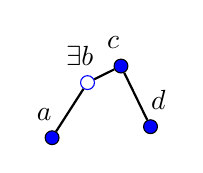
\begin{tikzpicture}
        \node[draw, circle, black, fill=blue, inner sep=0pt, minimum size=5pt,label={[xshift=-0.1cm, yshift=0.0cm]$a$}] (a) at (0,0) {};
        \node[draw, circle, blue,  inner sep=0pt, minimum size=5pt, label={[xshift=-0.1cm, yshift=0.0cm]$\exists b$}] (b) at (0.9*0.5,1*0.7) {};
        \node[draw, circle, black, fill=blue, inner sep=0pt, minimum size=5pt, label={[xshift=-0.1cm, yshift=0.0cm]$c$}] (c) at (1.75*0.5, 1.3*0.7) {};
        \node[draw, circle, black, fill=blue, inner sep=0pt, minimum size=5pt, label={[xshift=0.1cm, yshift=0.0cm]$d$}] (d) at (2.5*0.5,0.2*0.7) {};
    \draw[thick] (a) -- (b) -- (c) -- (d);
    \end{tikzpicture}
    \caption{}
    \label{fig:cap}
\end{subfigure}
\begin{subfigure}{0.2\textwidth}
    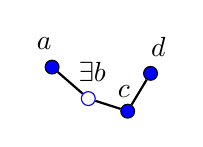
\begin{tikzpicture}
        \node[draw, circle, black, fill=blue, inner sep=0pt, minimum size=5pt,label={[xshift=-0.1cm, yshift=0.0cm]$a$}] (a) at (0,0) {};
        \node[draw, circle, blue,  inner sep=0pt, minimum size=5pt, label={[xshift=0.05cm, yshift=0.0cm]$\exists b$}] (b) at (0.92*0.5,-0.5*0.8) {};
        \node[draw, circle, black, fill=blue, inner sep=0pt, minimum size=5pt, label={[xshift=-0.05cm, yshift=-0.05cm]$c$}] (c) at (1.6*0.6, -0.7*0.8) {};
        \node[draw, circle, black, fill=blue, inner sep=0pt, minimum size=5pt, label={[xshift=0.1cm, yshift=0.0cm]$d$}] (d) at (2.5*0.5,-0.2*0.4) {};
    \draw[thick] (a) -- (b) -- (c) -- (d);
    \end{tikzpicture}
    \caption{}
    \label{fig:cup}
\end{subfigure}
\begin{subfigure}{0.2\textwidth}
    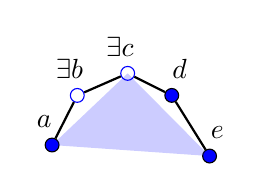
\begin{tikzpicture}
    \node[draw, circle, black, fill=blue, inner sep=0pt, minimum size=5pt,label={[xshift=-0.1cm, yshift=0.0cm]$a$}] (a) at (0,0) {};
    \node[draw, circle, blue,  inner sep=0pt, minimum size=5pt, label={[xshift=-0.1cm, yshift=0.0cm]$\exists b$}] (b) at (0.4*0.8,0.9*0.7) {};
    \node[draw, circle, blue, inner sep=0pt, minimum size=5pt, label={[xshift=-0.1cm, yshift=0.0cm]$\exists c$}] (c) at (1.2*0.8, 1.3*0.7) {};
    \node[draw, circle, black, fill=blue, inner sep=0pt, minimum size=5pt, label={[xshift=0.1cm, yshift=0.0cm]$d$}] (d) at (1.9*0.8,0.9*0.7) {};
    \node[draw, circle, black, fill=blue, inner sep=0pt, minimum size=5pt, label={[xshift=0.1cm, yshift=0.0cm]$e$}] (e) at (2.5*0.8,-0.2*0.7) {};

    \draw[thick] (a) -- (b) -- (c) -- (d) -- (e);
    \coordinate (a) at (0,0);
    \coordinate (c) at (1.2*0.8, 1.3*0.7);
    \coordinate (e) at (2.5*0.8,-0.2*0.7);
    \fill[blue, opacity=0.2] (a) -- (c) -- (e) -- cycle;
    \end{tikzpicture}
    \caption{}
    \label{fig:capF}
\end{subfigure}
\begin{subfigure}{0.2\textwidth}
    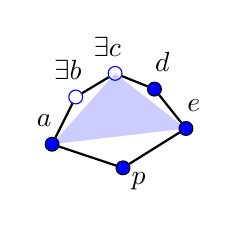
\begin{tikzpicture}
    \node[draw, circle, black, fill=blue, inner sep=0pt, minimum size=5pt,label={[xshift=-0.1cm, yshift=0.0cm]$a$}] (a) at (0,0) {};
    \node[draw, circle, blue,  inner sep=0pt, minimum size=5pt, label={[xshift=-0.1cm, yshift=0.0cm]$\exists b$}] (b) at (0.3,0.6) {};
    \node[draw, circle, blue, inner sep=0pt, minimum size=5pt, label={[xshift=-0.1cm, yshift=0.0cm]$\exists c$}] (c) at (0.8, 0.9) {};
    \node[draw, circle, black, fill=blue, inner sep=0pt, minimum size=5pt, label={[xshift=0.1cm, yshift=0.0cm]$d$}] (d) at (1.3,0.7) {};
    \node[draw, circle, black, fill=blue, inner sep=0pt, minimum size=5pt, label={[xshift=0.1cm, yshift=0.0cm]$e$}] (e) at (1.7,0.2) {};
    \node[draw, circle, black, fill=blue, inner sep=0pt, minimum size=5pt, label={[xshift=0.2cm, yshift=-0.5cm]$p$}] (p) at (0.9,-0.3) {};
    \draw[thick] (a) -- (b) -- (c) -- (d) -- (e) -- (p) -- (a);

    \coordinate (a) at (0,0);
    \coordinate (c) at (0.8, 0.9);
    \coordinate (e) at (1.7,0.2);
    \fill[blue, opacity=0.2] (a) -- (c) -- (e) -- cycle;
    \end{tikzpicture}
    \caption{}
    \label{fig:capFHexagon}
\end{subfigure}
\caption{Illustration of $4$-cap \textbf{(a)}, $4$-cup \textbf{(b)}, and $5$-cap \textbf{(c)} variables.}\label{fig:cup-cap-vars}
\end{figure}
